\documentclass[conference]{assets/latex/IEEEtran}

\usepackage{amsmath,amssymb,amsfonts}
\usepackage{graphicx}
\usepackage{textcomp}
\usepackage{xcolor}
\usepackage[backend=biber,style=numeric,url=false,isbn=false]{biblatex}
\addbibresource{assets/latex/report.bib}

\graphicspath{{assets/latex/}}

\begin{document}

\title{CS6524 Computer Vision Lab. 4\\ Optical Flow and Kalman Filters}

\author{\IEEEauthorblockN{Dara Heaphy}
\IEEEauthorblockA{\textit{Student ID 23369914} \\
University of Limerick}
\and
\IEEEauthorblockN{James Kelly}
\IEEEauthorblockA{\textit{Student ID XXXXXXXX} \\
University of Limerick}
}

\maketitle

\begin{abstract}
We track an object with Lucas-Kanade optical flow and use a constant-velocity
Kalman filter to predict it while hidden. The prediction was 59\,px off on
our own video and 188--345\,px off on the test videos, mostly because the
objects are only partly visible either side of the occluder.
\end{abstract}

% =====================================================================
\section{Methodology}

\textbf{Optical flow.} We track the median of the object's keypoints (px,
px/frame), since single points get lost and a mean is pulled by bad points. We seed points with \texttt{goodFeaturesToTrack}, with a
low quality level (0.005) because the potatoes and the ball have almost no
corners. Seeding is limited to a frame-difference mask to keep points off the
static background. LK uses a
$21\times21$ window and 3 pyramid levels, which copes with the ball's
$\sim$28\,px/frame. Points that don't come back within 1\,px when tracked backwards
are dropped, which removes points sliding onto the occluder edge. A point only joins the object once it has moved 4\,px, and
we keep the cluster of moving points with the most motion, so the hand
pushing the potato in 03 isn't picked instead.

\textbf{Kalman filter.} The state is $[x, y, v_x, v_y]$ with the usual
constant-velocity $F$ ($dt=1$\,frame) and no control input. Optical flow gives
us velocity for free, so we measure it too ($H=I_4$). $Q$ assumes a random acceleration of
$\sigma_a=0.5$\,px/frame$^2$. With 0.1--0.3 the filter wouldn't follow the
potato when the hand pushed it, and with $\ge 1$ it followed every jitter. $R$
is recomputed every frame from the spread of the keypoints, using the standard
error of the median ($1.25\,s/\sqrt{n}$). This was about 2--3$\times$ too
optimistic for velocity, so we added a minimum of 1\,px and 0.5\,px/frame.
$P_0$ is $R$ of the first measurement.

Just before the occluder only a sliver of the object is left and its
velocity is rubbish, so we reject velocities that fail a $\chi^2$ test (99.9\%)
against the prediction, and restart after 3 rejections in a row.

\textbf{Plotting.} After every occlusion of 10+ frames we split the track
into two (Fig.~\ref{fig:tr}). Trajectory 1 keeps correcting. Trajectory 2 starts from
the state just before the first new measurement and only predicts.

\begin{figure}[t]
\centerline{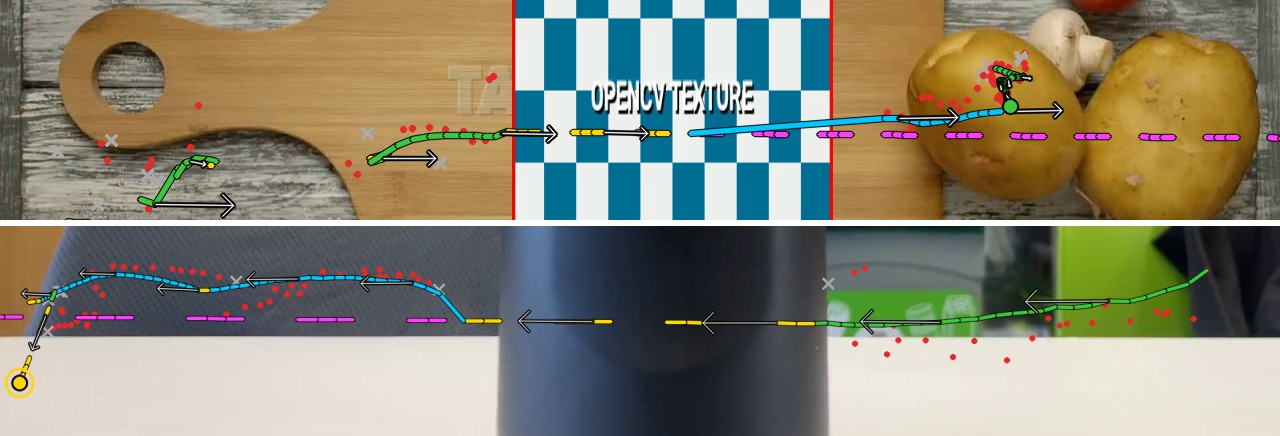
\includegraphics[width=\columnwidth]{tracking.jpg}}
\caption{Videos 03 (top) and 04 (bottom). Green: corrected; yellow: only
predicting; cyan: trajectory 1 after the object is back; magenta: trajectory 2
if it had not come back; red: measurements; grey crosses: rejected.}
\label{fig:tr}
\end{figure}

\begin{table}[t]
\caption{Prediction error when the object comes back}
\centering
\begin{tabular}{@{}lcccc@{}}
\hline
Video & Hidden & $v_x$ before & $v_x$ after & Error \\
\hline
01 & 26 fr & $-10.2$ & $-10.7$ & 345 px \\
02 & 76 fr & $\phantom{-}0.9$ & $\phantom{-}3.7$ & 295 px \\
03 & 17 fr & $\phantom{-}10.7$ & $\phantom{-}13.1$ & 188 px \\
04 (ours) & 19 fr & $-27.6$ & $-18.8$ & 59 px \\
\hline
\end{tabular}
\label{tab:res}
\end{table}

% =====================================================================
\section{Results and Discussion}
While the object is visible, $K_x$ sits around 0.08--0.17, so the filter mostly
trusts the model. While it's hidden, $P$ grows ($\sigma_x$ went from 1.5 to
42\,px in 01), so the first new measurement gets $K_x\approx0.9$--1.0 and the
estimate jumps onto it. Ten frames later $K_x$ is back to about 0.06.

\textbf{Partial visibility.} In 01 the speed hardly changes, but the error is
still 345\,px (Table~\ref{tab:res}). Going in, only the back of the orange is visible, so the median
point lags behind the real centre. Coming out, only the front is visible, so
it's ahead. Together that's roughly the size of the object, so the problem is
what we measure, not the filter. In 04 this partly cancels out the ball
slowing down (27.6 to 18.8\,px/frame), which we think is why it does best.

\textbf{Motion the model can't know about.} In 02 the pen goes in at
0.9\,px/frame and comes out 76 frames later higher up and four times faster.
In 03 the potato is pushed again while hidden. A constant-velocity model
can't predict either of these, but its uncertainty at least shows it:
$\sigma_x$ reached 194\,px in 02.

\textbf{What we'd do next.} Measure the centre of the motion-mask blob,
ignore partly visible frames, and model rolling objects slowing down.

\nocite{foundationsCVbook}
\printbibliography

\end{document}
